\hypertarget{evaluating-empirically-motivated-network-models}{%
\chapter{Evaluating Empirically-Motivated Network
Models}\label{evaluating-empirically-motivated-network-models}}

\usetikzlibrary{positioning,arrows,calc}
\tikzset{
    graph/.style={>=stealth,shorten >=1pt,shorten <=1pt,auto,node distance=1.5cm, semithick},
    world/.style={circle,draw,minimum size=0.5cm,fill=gray!15}, point/.style={circle,draw,inner sep=0.5mm,fill=black},
    model/.style={circle,draw,minimum size=0.5cm,fill=gray!20}, point/.style={circle,draw,inner sep=0.5mm,fill=black},
    reflexive above/.style={->,loop,looseness=7,in=120,out=60},
    reflexive below/.style={->,loop,looseness=7,in=240,out=300},
    reflexive left/.style={->,loop,looseness=7,in=150,out=210},
    reflexive right/.style={->,loop,looseness=7,in=30,out=330}
}

In this section, I turn my attention to actually using these
citation-based networks to evaluate Zollman's modeling efforts. It is
divided into three distinct investigations which each answer one of the
following questions:

\begin{enumerate}
\def\labelenumi{\arabic{enumi}.}
\tightlist
\item
  How does social network graph structure differ from the idealized
  models used by Zollman?
\item
  How do Zollman's results hold up on social network structure?
\item
  How can the new model behavior be characterized?
\end{enumerate}

\hypertarget{examining-graph-structure}{%
\section{Examining Graph Structure}\label{examining-graph-structure}}

The goal of this part is to show that there are important differences
between the MAG-derived empirical graphs and the canned cycle, wheel,
and complete graphs found in Zollman. However, before comparing these
graphs we must ensure that the output from the MAG from the prior
section fulfills all the requirements to work for the Bala-Goyal models
Zollman uses.

A key requirement of Bala-Goyal models is that the network is connected.
That is, every node can reach every other node. Intuitively, this is a
fine stipulation as an unreachable node is clearly outside of any
community represented by a graph. This can be seen in Figure
\ref{fig:disjoint} where two disjoint subgraphs \(A\) and \(B\) can be
separable from the combined graph \(A \cup B\).

\begin{figure}
    \centering
    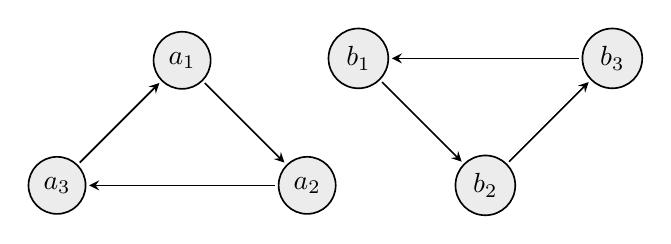
\begin{tikzpicture}[graph]
        \node[world] (a1) {$a_1$};
        \node[world] (a2) [below right=of a1] {$a_2$};
        \node[world] (a3) [below left=of a1] {$a_3$};

        \node[world] (b2) [right=of a2] {$b_2$};
        \node[world] (b3) [above right=of b2]{$b_3$};
        \node[world] (b1) [above left=of b2]{$b_1$};

        \path[->] (b1) edge (b2);
        \path[->] (b2) edge (b3);
        \path[->] (b3) edge (b1);
        \path[->] (a1) edge (a2);
        \path[->] (a2) edge (a3);
        \path[->] (a3) edge (a1);

    \end{tikzpicture}
    \caption{Two disconnected graphs, $A = \{ a_1, a_2, a_3 \}$, $B = \{ b_1, b_2, b_3 \}$. If we are studying the combined graph $A \cup B$, we'd be better off splitting the graph into $A$ and $B$ to be studied separately.}
    \label{fig:disjoint}
\end{figure}

The example in figure \ref{fig:disjoint} doesn't pose any issues for any
simulation run because both graphs will simply run independently, but
still correctly. However, problematic structures do commonly occur in
the MAG where information doesn't propagate or propagates only in one
direction, likely as a result of missing citations in the metadata.
Figure \ref{fig:isolate} demonstrates what this might look like where
isolated nodes would have no network effects and instead only rely on
their own random sampling. In practice, because agents are myopic and
pick whatever they think is successful, the initial random seed will
dictate the final action chosen because no data from neighbors ever
comes in.

\begin{figure}
    \centering
    \begin{tikzpicture}[graph]
        \node[world] (a1) {$a_1$};
        \node[world] (a2) [below right=of a1] {$a_2$};
        \node[world] (a3) [below left=of a1] {$a_3$};

        \node[world] (b1) [right=of a2] {$b_1$};
        \node[world] (b2) [above right=of b2]{$b_2$};
        \node[world] (c1) [above left=of b2]{$c_1$};

        \path[->] (b1) edge (b2);
        \path[->] (a1) edge (a2);
        \path[->] (a2) edge (a3);
        \path[->] (a3) edge (a1);

    \end{tikzpicture}
    \caption{Three disconnected graphs, $A = \{ a_1, a_2, a_3 \}$, $B = \{ b_1, b_2\}$, $C = \{c_1\}$. In this case, $c_1$ and $b_1$ experience no network effects at all because they have no neighbors.}
    \label{fig:isolate}
\end{figure}

To avoid these effects, I needed a construction that can take the
fragmented, large graphs and return the connected communities which lie
within them. The strongly connected component definition turned out to
be just that. If we recall from the previous section, a strongly
connected component is a subgraph of a larger graph where all nodes in
the subgraph are mutually reachable. In a strongly connected component,
every node has a neighbor. This stands in contrast to a weakly connected
component where all nodes simply must be reachable by some other node.
In the undirected graphs that Zollman used, these two definitions are
equivalent, however, because the citation relation is directed, I opt
for the strongly connected component to preserve the property that every
node has a neighbor. See Figure \ref{fig:3} for an example.

\begin{figure}
    \centering
    \begin{tikzpicture}[graph]
        \node[world] (a1) {$a_1$};
        \node[world] (a2) [below right=of a1] {$a_2$};
        \node[world] (a3) [below left=of a1] {$a_3$};

        \node[world] (b1) [right=of a2] {$b_1$};
        \node[world] (b2) [above right=of b2]{$b_2$};

        \path[->] (b1) edge[bend right] (b2);
        \path[->] (b2) edge[bend right] (b1);
        \path[->] (a2) edge (b1);
        \path[->] (a1) edge (a2);
        \path[->] (a2) edge (a3);
        \path[->] (a3) edge (a1);
    \end{tikzpicture}
    \caption{Strongly connected components are $A = \{ a_1, a_2, a_3 \}$ and $B = \{ b_1, b_2 \}$ whereas $A \cup B$ is a weakly connected component}
    \label{fig:3}
\end{figure}

So, given this definition, I further refine my graphs to be the strongly
connected components present in the field-specific graphs returned from
the MAG. As noted in the earlier section, there can be many strongly
connected components in a single field and these components can be quite
large. So, how do these components compare to the graphs Zollman used?
Figure \ref{fig:4} has examples of the cycle, wheel, and complete graphs
for reference. Note that these graphs can be scaled to any size
following the same patterns.

\begin{figure}
    \centering
    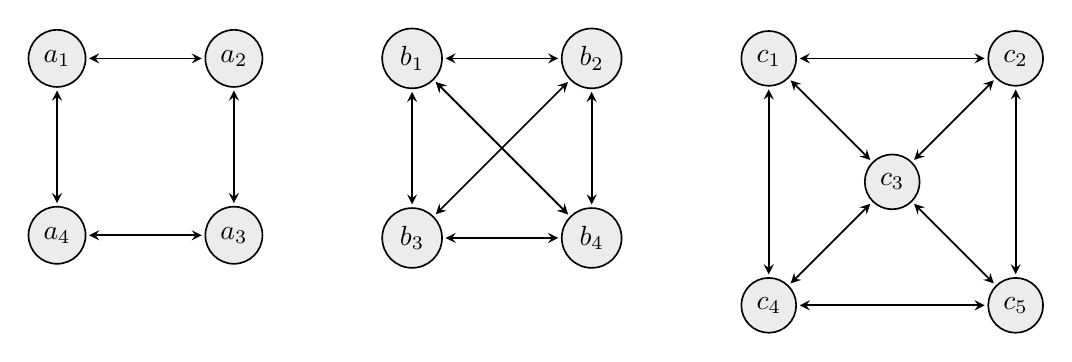
\begin{tikzpicture}[graph]
        \node[world] (a1) {$a_1$};
        \node[world] (a2) [right=of a1] {$a_2$};
        \node[world] (a3) [below=of a2] {$a_3$};
        \node[world] (a4) [below=of a1] {$a_4$};

        \node[world] (b1) [right=of a2] {$b_1$};
        \node[world] (b2) [right=of b1] {$b_2$};
        \node[world] (b3) [below=of b1] {$b_3$};
        \node[world] (b4) [below=of b2] {$b_4$};

        \node[world] (c1) [right=of b2] {$c_1$};
        \node[world] (c3) [below right=of c1] {$c_3$};
        \node[world] (c2) [above right=of c3] {$c_2$};
        \node[world] (c4) [below left=of c3] {$c_4$};
        \node[world] (c5) [below right=of c3] {$c_5$};

        \path[<->] (a1) edge (a2);
        \path[<->] (a2) edge (a3);
        \path[<->] (a3) edge (a4);
        \path[<->] (a4) edge (a1);

        \path[<->] (b1) edge (b2);
        \path[<->] (b1) edge (b3);
        \path[<->] (b1) edge (b4);
        \path[<->] (b2) edge (b3);
        \path[<->] (b2) edge (b4);
        \path[<->] (b3) edge (b4);
        \path[<->] (b4) edge (b1);

        \path[<->] (c1) edge (c2);
        \path[<->] (c2) edge (c5);
        \path[<->] (c5) edge (c4);
        \path[<->] (c4) edge (c1);
        \path[<->] (c1) edge (c3);
        \path[<->] (c2) edge (c3);
        \path[<->] (c4) edge (c3);
        \path[<->] (c5) edge (c3);
    \end{tikzpicture}
    \caption{Cycle $A = \{ a_1, a_2, a_3, a_4\}$, complete $B = \{ b_1, b_2, b_3, b_4 \}$ and wheel $C = \{ c_1, c_2, c_3, c_4, c_5 \}$}
    \label{fig:4}
\end{figure}

Now, given this understanding, I turn my attention back to understanding
how these collections of strongly-connected components from the
AuthorCites differ structurally from the synthetic graphs. The point of
this examination is to provide context that helps us understand the
simulation results as this structure should lead to those results.

To show how the wheel, cycle, and complete graphs differ, I first
created a scatter plot in Figure \ref{fig:nodesvdensity} which relates
the number of nodes and the density in each graph. Density is defined as
the number of actual edges over the number of potential edges in the
graph if it were a complete graph. The goal of plotting this
relationship is to ask if these empirical graphs have a similar
structure to any one of the synthetic graphs. Because complete graphs
are far denser than cycle and wheel graphs, I plotted this relationship
on a \(\log\)-\(\log\) plot to better visualize the differences between
them.

As it turned out, larger empirical graphs become much less dense as they
increase in size and are much closer to wheel graphs than to complete
graphs. Many fall in the wide region between wheel graphs and complete
graphs, indicating that there are many real communities in science which
have quite different density and structure than the synthetic graphs
discussed by Zollman. Furthermore, these differences grow as these
communities become larger because the quadratic growth of complete
graphs diverges from the more limited number of connections that any
given researcher could have.

What is important about this result is that the complete graph should be
regarded as a fairly unrealistic structure within larger research
communities. This result makes a lot of intuitive sense: as a community
grows in size, the ability of a single person to meaningfully read and
engage with others remains fixed. In a ten-person community, an author
might be able to read papers by everyone within that community, whereas
in a ten thousand person community authors will only be able to read,
let alone cite, a small fraction of that community. Thus, this
demonstrates that in the large communities that dominate today's global
research community, Zollman's dense complete networks are quite
unrealistic.

\begin{figure}
\hypertarget{fig:nodesvdensity}{%
\centering
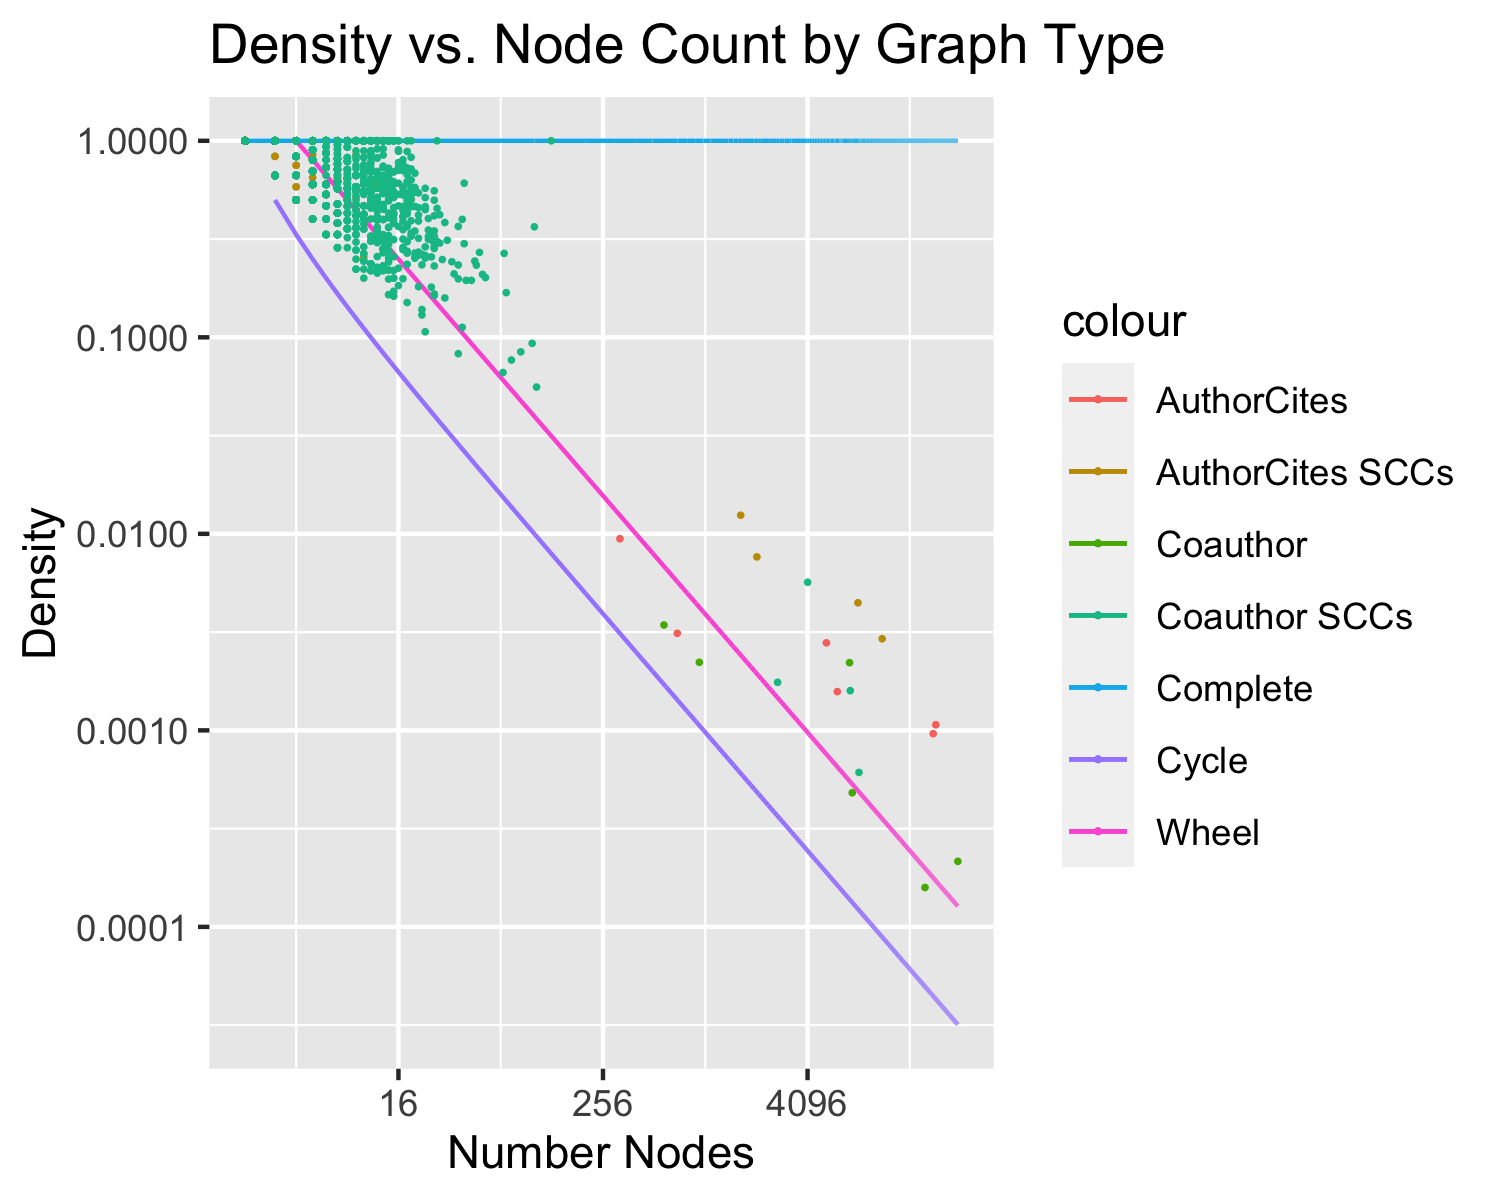
\includegraphics{figures/node_density_plot.png}
\caption{\(\log\) plot of graph density vs.~the number of nodes. Note
that the empirically constructed strongly-connected components decline
in density as they grow in size. This effect causes them to diverge from
the structure of complete graphs and begin to look much more like denser
versions of the cycle and wheel graphs.}\label{fig:nodesvdensity}
}
\end{figure}

Next, I decided to use a classic measure of graph structure, the degree
distribution, to show another critical way these . For the cycle and
complete graphs, every node either has two neighbors or \(n\) neighbors
for a graph of size \(n\). A wheel's edge nodes each have three
neighbors and the central node has \(n-1\) neighbors. This means the
degree of each node, the count of neighbors, doesn't vary from node to
node, which is a striking difference compared to real citations patterns
\ref{fig:degdist}.

\begin{figure}
\hypertarget{fig:degdist}{%
\centering
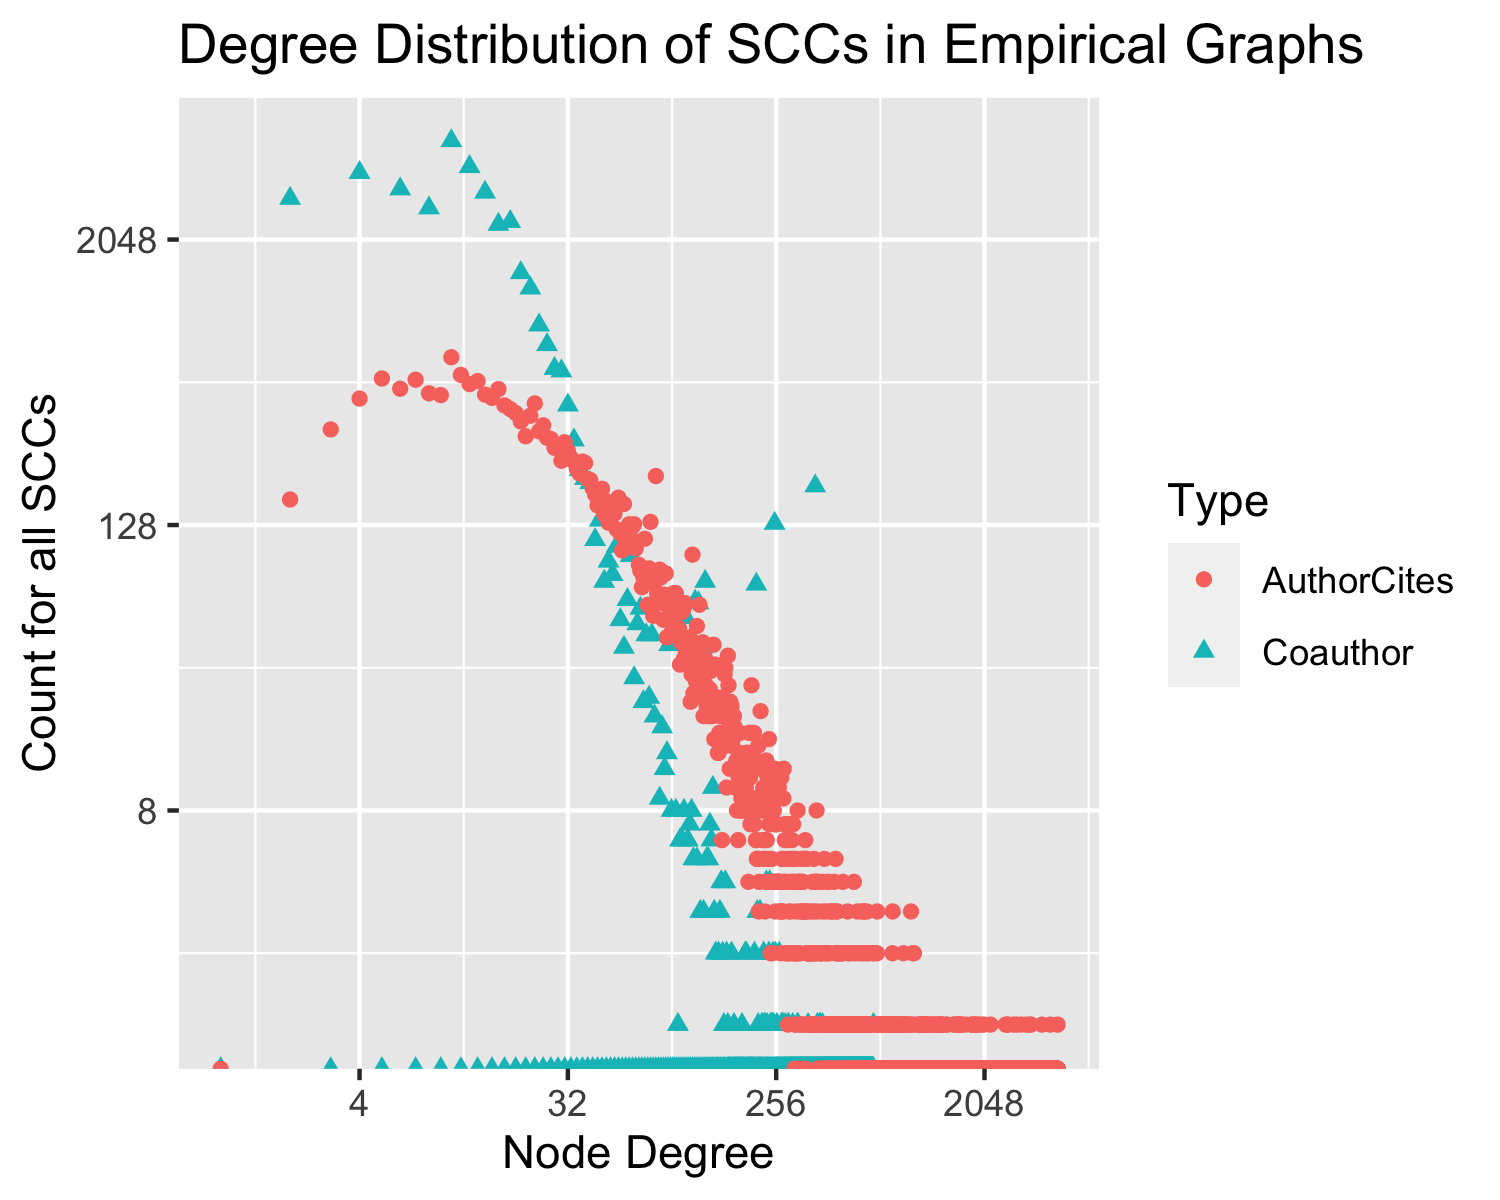
\includegraphics{figures/scc_degree_distribution.png}
\caption{\(\log\)-\(\log\) plot of degree distributions for empirical
SCC node degree counts that shows both AuthorCites and CoAuthor networks
roughly follow a power-law degree distribution. For context, cycle and
complete graphs are populated entirely with nodes with precisely the
same degree whereas, in the wheel graph, all but the central node has
the same degree. Thus, the citation graphs have distinctive diversity in
degree distribution compared with these synthetic
graphs.}\label{fig:degdist}
}
\end{figure}

Instead, this power-law distribution of real citation is what is often
called a ``small world'' distribution. These sorts of networks are
structure such that no two nodes are more than a few ``steps'' away from
each other, despite a lack of direct connections. The idea here is that
while you might have a small group of direct friends, the friends of
friends group and friends of friends of friends groups can be quite
large, encompassing many people thought to be complete strangers. The
conclusion to draw from this power-law effect is that this property is a
distinctive property of the graphs that is approximated, but not
replicated by any of the theoretical graphs.

\hypertarget{replicating-model-results}{%
\section{Replicating Model Results}\label{replicating-model-results}}

Now, given these graphs are notably different, how does Zollman's model
stack up on them? Do they behave like any of the synthetic graphs and,
if so, which ones? Furthermore, given that these graphs represent actual
communities, does the Zollman's noted effect where some denser
communities converge at a lower rate apply?

To begin to answer these questions, I ran Zollman's simulations on the
strongly-connected components from the AuthorCites graphs. I did not run
the simulations on the CoAuthor network because the co-authorship
relation does not map to communication in the sense that Zollman is
talking about. Collaboration is distinct from communication and Zollman
discusses the latter. Recall that in Zollman simulations, the model is
marked as ``converged'' successfully if and only if all agents chose the
action with a higher probability of success after the final model
iteration. Because this varies from run to run based on different random
seeds, Zollman often carries out repeated runs to approximate the
probability that the agents all converge.

To visualize the results of these simulations, I first plotted Zollman's
convergence metric relative to the density of the AuthorCites
strongly-connected components in figure \ref{fig:convergeprobdensity}.
This figure revealed that the same density-dependence relation Zollman
established still holds here. The least-dense real-world communities had
the highest probability of successful convergence on simulations.
However, the least-dense social network graphs are the largest ones. For
example, the field of peptic ulcer research contains a large strongly
connected component of low density that converged to the action with the
highest inherent probability of success on nearly every trial. Recall
that Zollman exhibited the field of peptic ulcer research as an example
of premature convergence leading to the wrong outcome. Thus, while
Zollman might have discovered a potential problem with a potential
solution in his models, the mechanisms in the model that led to that
problem seem notably different than those at play in these real-world
communities. For context, the large real-world communities converge
successfully with the same probability that Zollman observed in less
connected graphs.

On the other hand, there do exist many small groupings of 5-20 authors
that converge at lower rates due to high density. However, these
groupings don't have the influence that larger strongly-connected
components do because, by definition, they are not cited by anyone in
the primary connected component that makes up the bulk of the field in
most cases. This could be an interesting point for further structural
investigation of different fields as these smaller groupings have very
different structural properties than the larger graphs. Many of them are
nearly complete graphs. This could be due to a number of factors, such
as lab groupings which cause people to cite within a lab, lineages of
certain collaborations, etc. Determining why these are the case and
their prevalence in different fields of research would require more
careful empirical work by reading the papers involved and determining
what factors led to that structure. Deeper understanding here could help
shed light on how fragmented different fields are and what causes that
fragmentation.

\begin{figure}
\hypertarget{fig:convergeprobdensity}{%
\centering
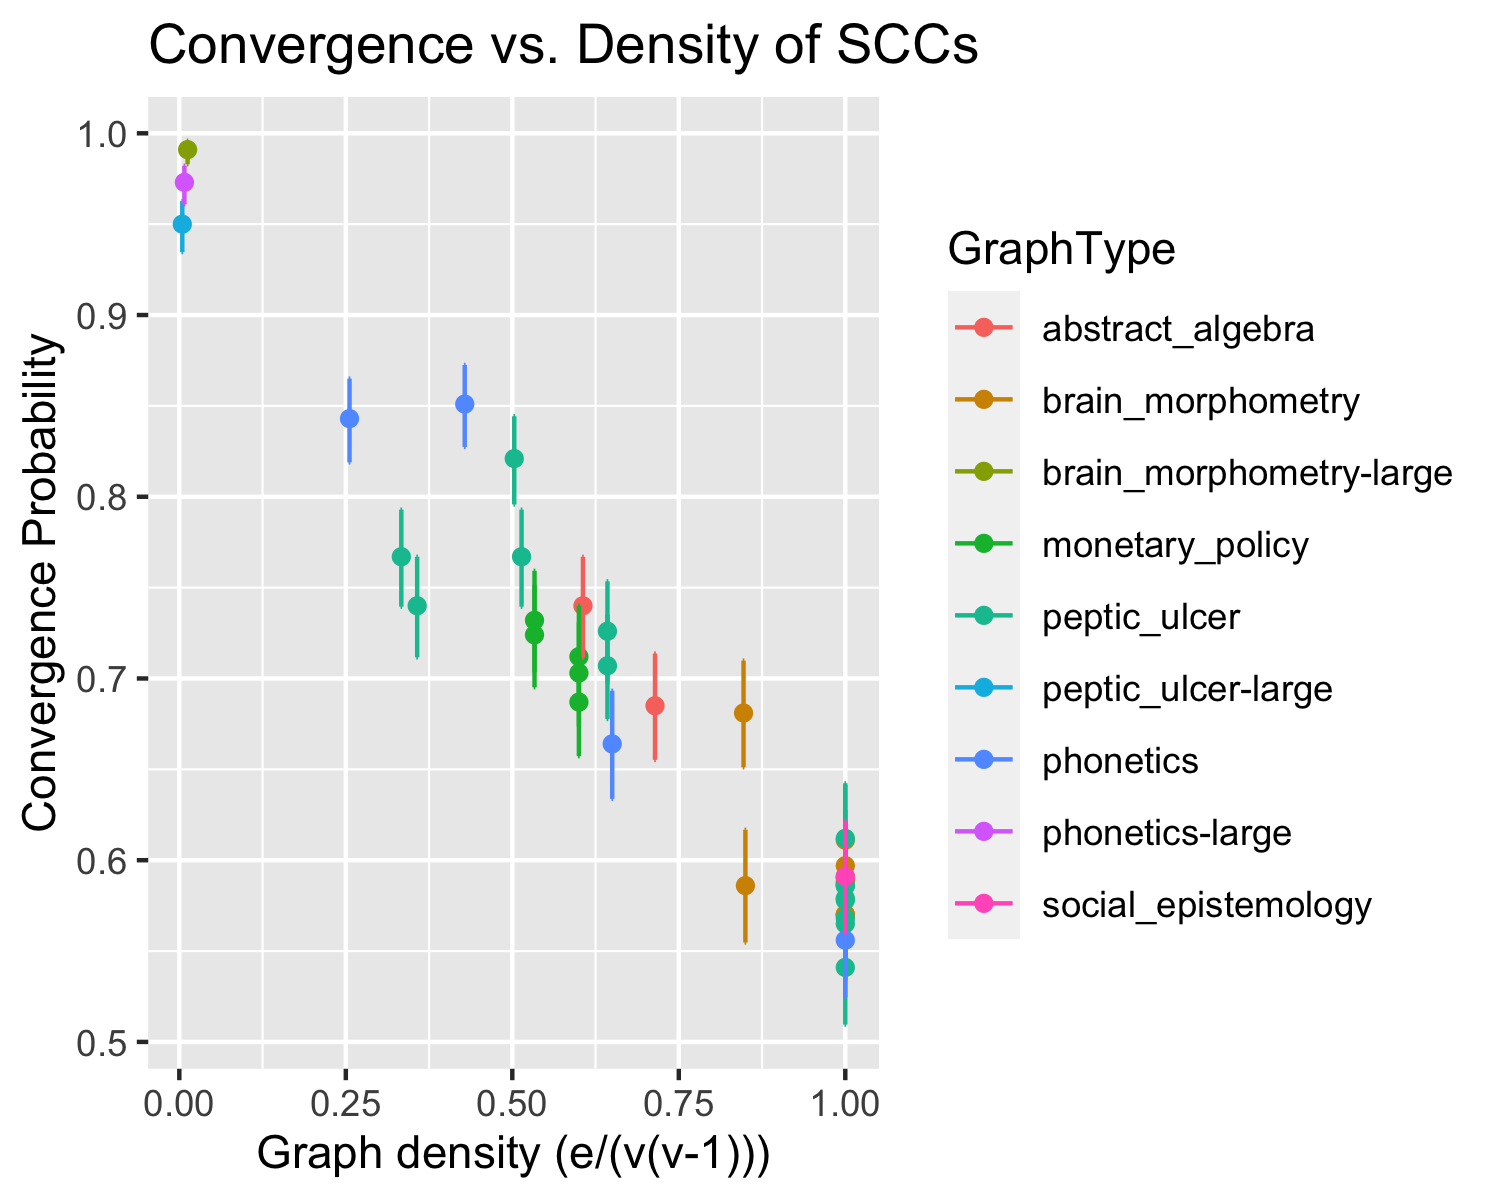
\includegraphics{figures/converge_prb_density.png}
\caption{Plot of successful convergence probability, as defined by
Zollman, against density for model runs on AuthorCites strongly
connected components. Graphs with more than 150 nodes are marked as
large. Note that all such large graphs are in the very top left corner
and have notably higher convergence probability. Each point has an
associated 95\% binomial confidence interval computed using the set of
trials.}\label{fig:convergeprobdensity}
}
\end{figure}

Next, I turned my attention to how fast the models converged on larger
graphs and what fraction of nodes end up selecting the right action at
each step. Do larger graphs converge more quickly? What fraction of
nodes get it right or wrong in the end? In figure
\ref{fig:convergespeed}, we see that large graphs converge very quickly
and completely, with very little variation in the fraction of nodes that
end up converged. Smaller graphs, on the other hand, have quite a bit
more variation partly because a single incorrect node has a bigger
impact on the overall network when that network is small. One node wrong
in four is a major schism whereas one node wrong in two-thousand is an
outlier.

\begin{figure}
\hypertarget{fig:convergespeed}{%
\centering
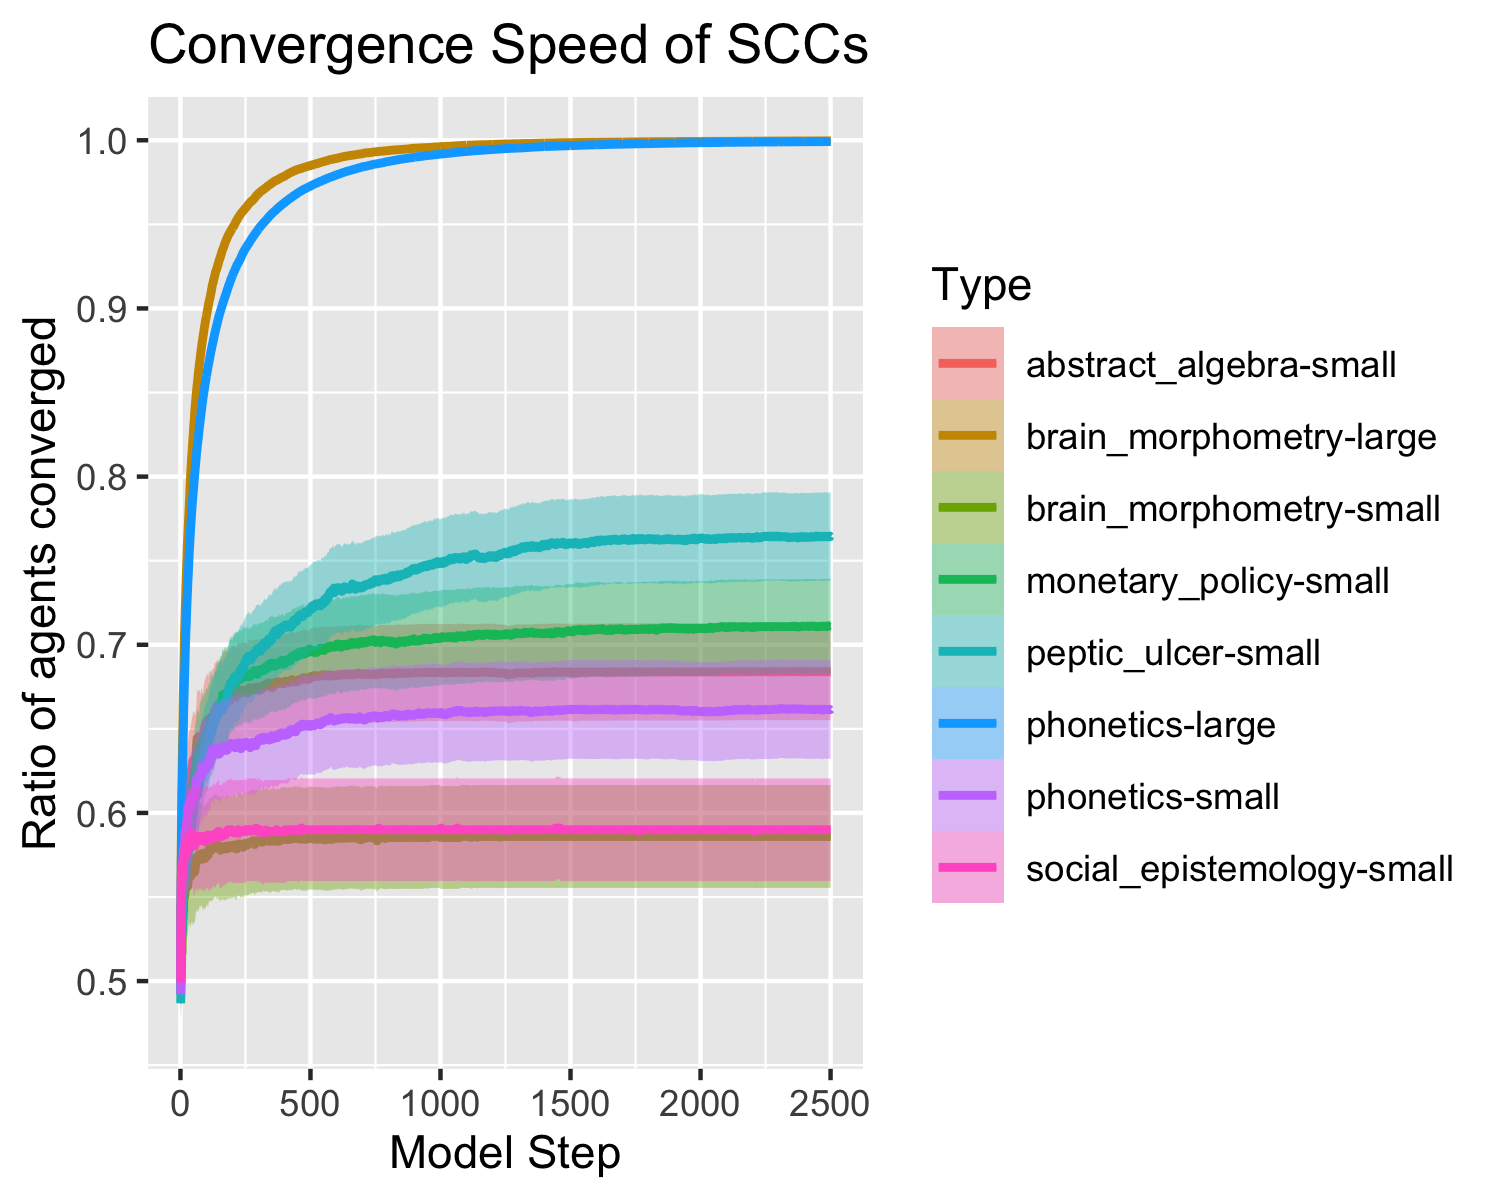
\includegraphics{figures/converge_speed.png}
\caption{Graph showing the convergence by step. The lines shown are the
mean ratio of agents converged at that given step with a 95\% confidence
interval shown as a band around each line. Very large, sparse graphs
quickly converge to complete agreement. Small dense graphs converge more
slowly to a plateau. The mean and confidence interval metric does not
capture that smaller graphs also jump out of that plateau and converge
rapidly when then do converge, though that happens at a much lower rate
that the large graphs.}\label{fig:convergespeed}
}
\end{figure}

\hypertarget{characterizing-model-behavior}{%
\section{Characterizing Model
Behavior}\label{characterizing-model-behavior}}

While the graphs of convergence probabilities and densities quantify the
behavior of the model and allow for rigorous conclusions, they don't
give a good intuitive idea of what a model \emph{looks} like. To rectify
this, figure \ref{fig:pepticprog} presents a pictorial view of a single
model run of the simulation on the peptic ulcer graph. To do this, I
used the standard ``spring'' layout algorithm to visualize the graph
structure and recolored each node according to its selected action at
each step. Nodes can be seen slowly flipping back and forth between the
two actions but the simulation eventually converges and all agents agree
on the right action. This happens rapidly because the peptic ulcer graph
is large and sparse. The spring layout shows that one part of peptic
ulcer work is denser than the other and thus that dense core converges
slightly faster than the rest of the graph before propagating out to all
nodes at the peripheries. Nodes in the middle generally have a higher
degree while nodes at the edges have a lower degree, so this is
consistent with the most well-connected authors converging first to a
new trend with less connected authors adopting that theory much later.

\begin{figure}
\hypertarget{fig:pepticprog}{%
\centering
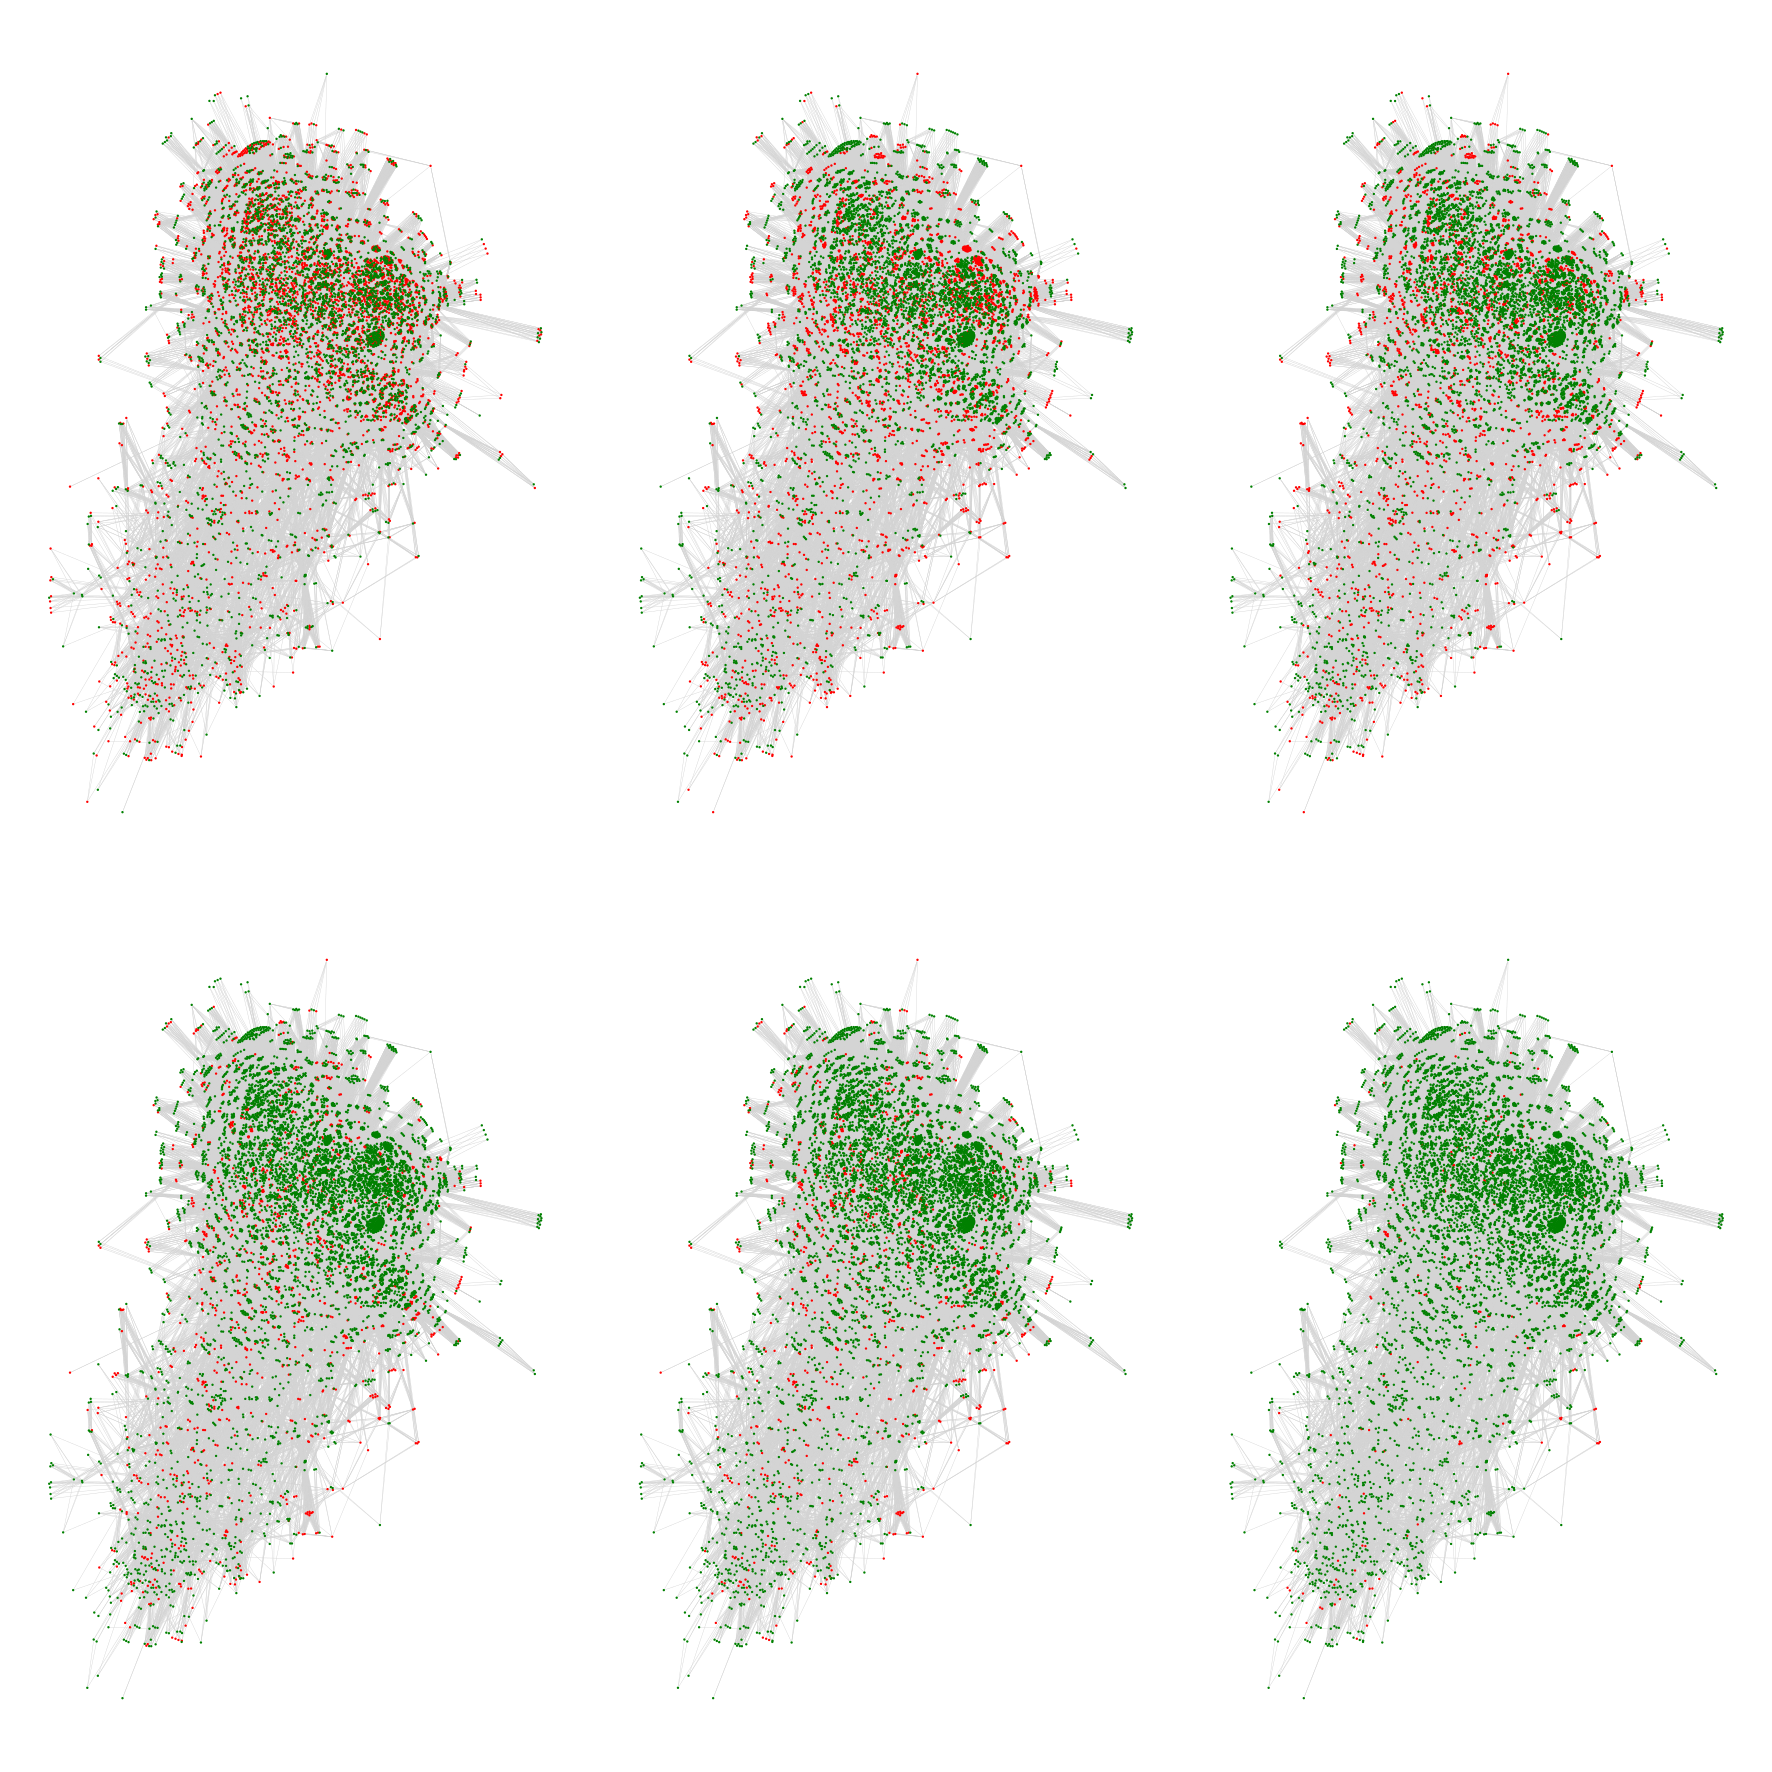
\includegraphics{figures/peptic_ulcer_1-5-10-50-100-500.png}
\caption{Frames from a model run on the large peptic ulcer strongly
connected component. Each plot shows that state of the model at a given
step where red nodes have chosen the suboptimal theory and green nodes
the optimal one. The first row contains the initial state, the state
after the 5th step and the one after the 10th. The second has the 50th,
the 100th, and the 500th. The simulation continues on to 10,000 steps
where all nodes are green, but nearly all nodes have chosen correctly by
step 500 on the peptic ulcer graph because it is large and
sparse.}\label{fig:pepticprog}
}
\end{figure}

\hypertarget{experimental-conclusions-and-takeaways}{%
\section{Experimental Conclusions and
Takeaways}\label{experimental-conclusions-and-takeaways}}

Overall, the empirically-simulated models largely converged at rates
that Zollman's findings would have predicted based on the
graph-theoretic properties of the AuthorCites graphs. Lower density
graphs converged more completely than higher density ones, which is
consistent with Zollman's findings. However, the large, less-dense
graphs also converged faster than their denser counterparts, which calls
into question one of Zollman's worries: that less density and less
communication can lead to slower convergence which delays science.

In reality, these less dense graphs are substantially less dense than
any complete graph, but are much denser than the cycle and wheel graphs
that Zollman tests against. The ``small world'' effect also means that
pair-wise distances between nodes are short and thus information never
has that far to travel between nodes. This effect differs quite a bit
from the cycle graph which forces agents to play telephone with their
results, slowing convergence substantially.

Most importantly, these results call into question Zollman's
recommendation for less communication to avoid premature convergence.
The answer must be much more nuanced than this given these results.
First of all, the scholarly graphs are for the most part not that dense
already and they converge at high rates as Zollman predicts. Secondly,
they also happen to converge faster than small dense graphs, indicating
that there is no price paid for that high rate of successful
convergence. In short, real-world ``small world'' graphs get the best of
both worlds under Zollman's metrics.

However, this means that these effects cannot explain why the peptic
ulcer field converged prematurely because that field is fairly well
structured for Zollman's model. Zollman's model would predict that
problematic fields like peptic ulcer research would be too dense and
converge to the wrong answer too quickly. However, because the peptic
ulcer graph turned out to not be very dense, it converged quickly to the
right answer, meaning the Zollman's model doesn't explain why peptic
ulcer research in the real world converged on the wrong answer. Thus,
some other mechanism than the one modeled must be at play.

Furthermore, there is a sense in which the problem here is not enough
communication. For example, the strongly connected components that were
small and very dense can counterintuitively lower the overall density of
the large graph by joining it. This means that had some of those dense
components joined the larger, primary component of the field, the field
likely would maintain the same fast and accurate convergence that the
larger component had from the start. Thus, the answer cannot be as
simple as a blanket recommendation of less or more density, rather, some
groups who are separated from the overall community might benefit from
being looped in with the mainstream. Furthermore, those in the
mainstream would do better by reaching out and forming new connections
with these disconnected groups than by densifying the large central
component further.

So, this empirical work suggests the while Zollman's theoretical results
hold, their application to real data changes our understanding of what
those results mean for the actual world. Because I wanted the comparison
with Zollman's work to be direct, I mirrored his model structure exactly
but for the empirical graphs. This highlights how empirical grounding
changes conclusions, however, it also means my work likely suffers from
all the same mathematical stability problems identified by Rosenstock,
Bruner, and O'Connor \autocite{rosenstockEpistemicNetworksLess2017a}.
Essentially, the model is not robust to changes in non-graph parameters,
like the underlying binomial probabilities of the actions and the
initial priors for each individual. An interesting follow-up project
might be to determine if this sensitivity is reduced to some extent on
the more robust ``small world'' graphs.
